\PassOptionsToPackage{unicode}{hyperref}
\PassOptionsToPackage{hyphens}{url}
\PassOptionsToPackage{dvipsnames,svgnames,x11names}{xcolor}
\documentclass[
  spanish,
  11pt,
  a4paper,
  DIV=11,
  numbers=noendperiod]{scrartcl}

\usepackage{xcolor}
\usepackage[top=24mm,bottom=24mm,left=24mm,right=24mm,headheight=15pt,headsep=8mm]{geometry}
\usepackage{amsmath,amssymb}
\usepackage{iftex}
\ifPDFTeX
  \usepackage[T1]{fontenc}
  \usepackage[utf8]{inputenc}
  \usepackage{textcomp}
\else
  \usepackage{unicode-math}
  \defaultfontfeatures{Scale=MatchLowercase}
  \defaultfontfeatures[\rmfamily]{Ligatures=TeX,Scale=1}
\fi
\usepackage{lmodern}
\IfFileExists{upquote.sty}{\usepackage{upquote}}{}
\IfFileExists{microtype.sty}{
  \usepackage[]{microtype}
  \UseMicrotypeSet[protrusion]{basicmath}
}{}
\usepackage{graphicx}
\usepackage{float}
\usepackage[bidi=basic]{babel}
\let\LanguageShortHands\languageshorthands
\def\languageshorthands#1{}
\setlength{\emergencystretch}{3em}
\setcounter{secnumdepth}{5}
\providecommand{\tightlist}{\setlength{\itemsep}{0pt}\setlength{\parskip}{0pt}}

\newcommand{\practicaPdfCoverImage}{}
% PDF style for Practica 9.
% A modest university handout look: classical type, clear hierarchy,
% restrained color, and durable code/callout styling.

\usepackage{graphicx}
\usepackage[export]{adjustbox}
\usepackage{fontspec}
\usepackage{microtype}
\usepackage{scrlayer-scrpage}
\usepackage{tikz}
\usepackage{fvextra}
\usepackage{caption}
\usepackage{subcaption}
\usepackage[skins,breakable]{tcolorbox}

\providecommand{\practicaPdfCoverImage}{}

\definecolor{uzaInk}{HTML}{172033}
\definecolor{uzaMuted}{HTML}{5F6B7A}
\definecolor{uzaBlue}{HTML}{1F5F8B}
\definecolor{uzaBlueDark}{HTML}{153E5C}
\definecolor{uzaCyan}{HTML}{EAF4F7}
\definecolor{uzaLine}{HTML}{D7E2EA}
\definecolor{uzaCodeBg}{HTML}{F5F7F9}
\definecolor{uzaTip}{HTML}{237A57}
\definecolor{uzaWarn}{HTML}{A65F00}

\IfFontExistsTF{TeX Gyre Pagella}{
  \setmainfont{TeX Gyre Pagella}
}{}
\IfFontExistsTF{TeX Gyre Heros}{
  \setsansfont{TeX Gyre Heros}
}{}
\IfFontExistsTF{TeX Gyre Cursor}{
  \setmonofont{TeX Gyre Cursor}[Scale=0.86]
}{
  \setmonofont{Latin Modern Mono}[Scale=0.88]
}

\KOMAoptions{parskip=half}
\setlength{\parindent}{0pt}
\setlength{\parskip}{0.55em plus 0.15em minus 0.08em}
\linespread{1.035}

\addtokomafont{disposition}{\sffamily\color{uzaBlueDark}}
\addtokomafont{section}{\LARGE}
\addtokomafont{subsection}{\Large}
\addtokomafont{subsubsection}{\normalsize\bfseries}
\RedeclareSectionCommand[beforeskip=2.2em plus 0.4em minus 0.2em,afterskip=1.0em]{section}
\RedeclareSectionCommand[beforeskip=1.2em,afterskip=0.55em]{subsection}
\RedeclareSectionCommand[beforeskip=1.0em,afterskip=0.35em]{subsubsection}

\clearpairofpagestyles
\automark[section]{section}
\ihead{\sffamily\footnotesize\textcolor{uzaMuted}{Informática (30717)}}
\ohead{\sffamily\footnotesize\textcolor{uzaMuted}{\headmark}}
\cfoot{\sffamily\small\textcolor{uzaMuted}{\pagemark}}
\setkomafont{pageheadfoot}{\normalfont}
\KOMAoptions{headsepline=0.35pt}
\addtokomafont{headsepline}{\color{uzaLine}}

\makeatletter
\AtBeginDocument{%
  \hypersetup{
    linkcolor=uzaBlueDark,
    urlcolor=uzaBlue,
    citecolor=uzaBlueDark
  }%
  \@ifundefined{Highlighting}{%
    \DefineVerbatimEnvironment{Highlighting}{Verbatim}{
      commandchars=\\\{\},
      fontsize=\small,
      breaklines=true,
      breakanywhere=true
    }%
  }{%
    \RecustomVerbatimEnvironment{Highlighting}{Verbatim}{
      commandchars=\\\{\},
      fontsize=\small,
      breaklines=true,
      breakanywhere=true
    }%
  }%
  \@ifundefined{Shaded}{%
    \newenvironment{Shaded}{%
      \begin{tcolorbox}[
        enhanced,
        breakable,
        sharp corners,
        boxrule=0.25pt,
        colback=uzaCodeBg,
        colframe=uzaLine,
        borderline west={1.4pt}{0pt}{uzaBlue},
        left=2mm,
        right=2mm,
        top=1.4mm,
        bottom=1.4mm,
        before skip=0.75em,
        after skip=0.75em
      ]%
    }{%
      \end{tcolorbox}%
    }%
  }{%
    \renewenvironment{Shaded}{%
      \begin{tcolorbox}[
        enhanced,
        breakable,
        sharp corners,
        boxrule=0.25pt,
        colback=uzaCodeBg,
        colframe=uzaLine,
        borderline west={1.4pt}{0pt}{uzaBlue},
        left=2mm,
        right=2mm,
        top=1.4mm,
        bottom=1.4mm,
        before skip=0.75em,
        after skip=0.75em
      ]%
    }{%
      \end{tcolorbox}%
    }%
  }%
}
\makeatother

\newcommand{\PracticeCode}[1]{%
  \begin{Shaded}%
  \VerbatimInput[
    fontsize=\small,
    breaklines=true,
    breakanywhere=true
  ]{#1}%
  \end{Shaded}%
}

\makeatletter
\renewcommand{\maketitle}{%
  \begin{titlepage}
    \thispagestyle{empty}
    \begin{tikzpicture}[remember picture,overlay]
      \fill[uzaCyan] (current page.north west) rectangle ([yshift=-72mm]current page.north east);
      \fill[uzaBlue] (current page.north west) rectangle ([xshift=7mm]current page.south west);
    \end{tikzpicture}
    \vspace*{12mm}
    {\sffamily\small\bfseries\textcolor{uzaBlue}{INFORMÁTICA (30717)}}\par
    \vspace{5mm}
    {\sffamily\bfseries\fontsize{30}{35}\selectfont\textcolor{uzaInk}{\@title}}\par
    \vspace{3mm}
    {\sffamily\Large\textcolor{uzaMuted}{Grado en Estudios en Arquitectura}}\par
    \vspace{8mm}
    {\color{uzaBlue}\rule{\textwidth}{0.6pt}}\par
    \if\relax\detokenize\expandafter{\practicaPdfCoverImage}\relax
    \else
      \vspace{5mm}
      {\centering\includegraphics[width=\textwidth,height=78mm,keepaspectratio]{\practicaPdfCoverImage}\par}
    \fi
    \vfill
    {\sffamily\large\textcolor{uzaBlueDark}{Universidad de Zaragoza}}\par
    \vspace{2mm}
    {\sffamily\small\textcolor{uzaMuted}{Material de prácticas del curso 2025--2026}}\par
  \end{titlepage}
}
\makeatother

\captionsetup{
  font={small,sf},
  labelfont={bf,color=uzaBlueDark},
  textfont={color=uzaInk},
  justification=centering,
  singlelinecheck=false,
  skip=6pt
}
\captionsetup[subfigure]{
  font={small,sf},
  labelfont={bf,color=uzaBlueDark},
  justification=centering,
  singlelinecheck=true,
  skip=4pt
}

\newcommand{\PracticeCredit}[1]{\textcolor{uzaMuted}{#1}}
\newcommand{\PracticeImagePair}[6]{%
  \begin{figure}[tbp]
    \centering
    \begin{minipage}[t]{0.485\linewidth}
      \includegraphics[width=\linewidth]{#3}
      \vspace{2mm}
      \centering{\sffamily\footnotesize #4}
    \end{minipage}\hfill
    \begin{minipage}[t]{0.485\linewidth}
      \includegraphics[width=\linewidth]{#5}
      \vspace{2mm}
      \centering{\sffamily\footnotesize #6}
    \end{minipage}
    \caption{\label{#1}#2}
  \end{figure}
}

\renewcommand{\arraystretch}{1.16}
\setlength{\tabcolsep}{6pt}
\setkeys{Gin}{center}

% Quarto callout colors are referenced by generated tcolorbox options.
% Apply them at document start so they win over Quarto's defaults.
\AtBeginDocument{%
  \definecolor{quarto-callout-note-color}{HTML}{1F5F8B}%
  \definecolor{quarto-callout-note-color-frame}{HTML}{1F5F8B}%
  \definecolor{quarto-callout-tip-color}{HTML}{237A57}%
  \definecolor{quarto-callout-tip-color-frame}{HTML}{237A57}%
  \definecolor{quarto-callout-warning-color}{HTML}{A65F00}%
  \definecolor{quarto-callout-warning-color-frame}{HTML}{A65F00}%
  \definecolor{quarto-callout-important-color}{HTML}{9B2C2C}%
  \definecolor{quarto-callout-important-color-frame}{HTML}{9B2C2C}%
  \definecolor{quarto-callout-caution-color}{HTML}{B45309}%
  \definecolor{quarto-callout-caution-color-frame}{HTML}{B45309}%
}

\KOMAoption{captions}{tableheading}
\usetikzlibrary{arrows.meta}

\newtcolorbox{PracticeWarningBox}[1]{%
  enhanced,
  breakable,
  sharp corners,
  boxrule=0.25pt,
  colback=white,
  colframe=uzaLine,
  colbacktitle=uzaCyan,
  coltitle=uzaInk,
  fonttitle=\sffamily\bfseries,
  title={#1},
  borderline west={1.4pt}{0pt}{uzaWarn},
  left=2mm,
  right=2mm,
  top=1.4mm,
  bottom=1.4mm,
  before skip=0.75em,
  after skip=0.75em
}

\newtcolorbox{PracticeImportantBox}[1]{%
  enhanced,
  breakable,
  sharp corners,
  boxrule=0.25pt,
  colback=white,
  colframe=uzaLine,
  colbacktitle=uzaCyan,
  coltitle=uzaInk,
  fonttitle=\sffamily\bfseries,
  title={#1},
  borderline west={1.4pt}{0pt}{red!55!black},
  left=2mm,
  right=2mm,
  top=1.4mm,
  bottom=1.4mm,
  before skip=0.75em,
  after skip=0.75em
}

\usepackage{bookmark}
\IfFileExists{xurl.sty}{\usepackage{xurl}}{}
\urlstyle{same}
\hypersetup{
  pdftitle={Práctica 6: Resolución de problemas en Java (III)},
  pdflang={es},
  colorlinks=true,
  linkcolor={uzaBlueDark},
  filecolor={Maroon},
  citecolor={Blue},
  urlcolor={uzaBlue},
  pdfcreator={LaTeX}
}

\title{Práctica 6: Resolución de problemas en Java (III)}
\author{}
\date{}

\begin{document}
\maketitle

\renewcommand*\contentsname{Tabla de contenidos}
{
\hypersetup{linkcolor=}
\setcounter{tocdepth}{2}
\tableofcontents
}

\clearpage

\section{Objetivos de la práctica}\label{objetivos-de-la-practica}

Los objetivos de la sexta práctica de la asignatura son los siguientes:

\begin{itemize}
\tightlist
\item Desarrollar algoritmos en Java.
\item Ejecutar algoritmos en el entorno \emph{Eclipse}.
\end{itemize}

\section{Algoritmos de ordenación}\label{algoritmos-de-ordenacion}

Dado un vector de \(n\) números enteros, el objetivo de esta práctica es implementar dos algoritmos de ordenación: el algoritmo de \textbf{ordenación de burbuja} (\emph{bubble sort}) y el algoritmo de \textbf{selección} (\emph{selection sort}). Ambos algoritmos son métodos sencillos para ordenar una lista de elementos, aunque no son los más eficientes para grandes conjuntos de datos. Sin embargo, son útiles para entender los conceptos básicos de ordenación y complejidad algorítmica.

\section{\texorpdfstring{\emph{Bubble sort} u ordenación de burbuja}{Bubble sort u ordenación de burbuja}}\label{bubble-sort-u-ordenacion-de-burbuja}

El algoritmo de \textbf{ordenación de burbuja} funciona \textbf{comparando cada par de elementos adyacentes} e \textbf{intercambiándolos si están en el orden incorrecto}. Este proceso se repite hasta que la lista está completamente ordenada.

Para un vector de \(n\) números enteros, el proceso es:

\begin{itemize}
\tightlist
\item Comparamos \(v[0]\) con \(v[1]\) y, si es mayor, los intercambiamos.
\item Repetimos la comparación con cada par de elementos adyacentes hasta llegar a \(v[n-2]\) y \(v[n-1]\).
\item En ese momento, la última posición ya está ordenada.
\item Repetimos el proceso hasta tener todo el vector ordenado.
\item Si en un recorrido completo no hay ningún intercambio, el vector ya está ordenado.
\end{itemize}

\begin{figure}[H]
\centering
\begin{tikzpicture}[x=1cm,y=1cm, every node/.style={font=\sffamily\small}]
  \draw[rounded corners=2pt, fill=uzaCodeBg, draw=uzaLine] (-0.6,-0.35) rectangle (8.45,3.05);
  \node[anchor=west,color=uzaBlueDark,font=\sffamily\bfseries] at (0,2.62) {Primera pasada};
  \foreach \x/\value/\fillcolor in {0/37/uzaWarn,1/18/uzaWarn,2/42/uzaTip,3/25/uzaTip,4/73/uzaBlue,5/91/uzaBlue,6/12/uzaTip,7/66/uzaTip} {
    \draw[rounded corners=2pt, fill=\fillcolor, draw=white, line width=1.2pt] (\x,0.92) rectangle ++(0.92,0.92);
    \node[color=white, font=\sffamily\bfseries] at (\x+0.46,1.38) {\value};
  }
  \node[anchor=east,color=uzaMuted,font=\sffamily\bfseries] at (-0.14,1.38) {\texttt{v}};
  \draw[<->, >=Latex, color=uzaWarn, thick] (0.46,2.04) -- (1.46,2.04);
  \node[fill=white, inner sep=1.5pt, text=uzaWarn] at (0.96,2.28) {comparar};
  \draw[color=uzaBlueDark, thick] (4.02,0.66) -- (5.92,0.66);
  \node[anchor=north,color=uzaBlueDark] at (4.97,0.48) {zona ya ordenada};
\end{tikzpicture}
\caption{Idea visual de una iteración de ordenación de burbuja. La versión web y las diapositivas permiten avanzar paso a paso.}\label{fig-burbuja-estatica}
\end{figure}

\section{\texorpdfstring{\emph{Selection sort} u ordenación por selección}{Selection sort u ordenación por selección}}\label{selection-sort-u-ordenacion-por-seleccion}

El algoritmo de ordenación por \textbf{selección} funciona \textbf{dividiendo la lista en dos partes}: la parte \textbf{ordenada} y la parte \textbf{no ordenada}. En cada iteración, el algoritmo selecciona el elemento más pequeño de la parte no ordenada y lo intercambia con el primer elemento de esa parte.

El proceso es:

\begin{itemize}
\tightlist
\item Buscamos el elemento más pequeño en el vector y lo intercambiamos con el primer elemento.
\item Después buscamos el elemento más pequeño en el resto del vector y lo intercambiamos con el segundo elemento.
\item Repetimos este proceso hasta que todo el vector esté ordenado.
\end{itemize}

\begin{figure}[H]
\centering
\begin{tikzpicture}[x=1cm,y=1cm, every node/.style={font=\sffamily\small}]
  \draw[rounded corners=2pt, fill=uzaCodeBg, draw=uzaLine] (-0.6,-0.35) rectangle (8.45,3.18);
  \node[anchor=west,color=uzaBlueDark,font=\sffamily\bfseries] at (0,2.72) {B\'usqueda del menor};
  \foreach \x/\value/\fillcolor in {0/12/uzaBlue,1/18/uzaBlue,2/42/uzaTip,3/25/uzaWarn,4/73/uzaTip,5/91/uzaTip,6/37/uzaTip,7/66/uzaTip} {
    \draw[rounded corners=2pt, fill=\fillcolor, draw=white, line width=1.2pt] (\x,0.82) rectangle ++(0.92,0.92);
    \node[color=white, font=\sffamily\bfseries] at (\x+0.46,1.28) {\value};
  }
  \node[anchor=east,color=uzaMuted,font=\sffamily\bfseries] at (-0.14,1.28) {\texttt{v}};
  \draw[color=uzaBlueDark, thick] (0.02,2.06) -- (1.92,2.06);
  \node[fill=white, inner sep=1.5pt, text=uzaBlueDark] at (0.78,2.31) {zona ordenada};
  \draw[-{Latex[length=2mm]}, color=uzaWarn, thick] (3.46,2.06) -- (2.46,2.06);
  \node[fill=white, inner sep=1.5pt, text=uzaWarn] at (3.35,2.31) {m\'inimo provisional};
\end{tikzpicture}
\caption{Idea visual de una iteración de ordenación por selección. La versión web y las diapositivas muestran las comparaciones paso a paso.}\label{fig-seleccion-estatica}
\end{figure}

\section{Ejercicios}\label{ejercicios}

Implementa los algoritmos de ordenación de burbuja y selección en Java utilizando dos clases diferentes, \texttt{OrdenacionBurbuja.java} y \texttt{OrdenacionSeleccion.java}. La siguiente estructura puede servir como punto de partida para la clase de burbuja:

\PracticeCode{../resources/practica6/snippets/java/ordenacion-burbuja-template.java}

Ejecuta paso a paso los algoritmos utilizando el depurador de \emph{Eclipse} para entender cómo funciona el proceso de ordenación. Utiliza un tamaño de vector pequeño, por ejemplo 20 elementos, para facilitar la visualización del proceso. Además, debes \textbf{medir el tiempo de ejecución} de los algoritmos utilizando cuatro valores de \(n\): \(10^2\), \(10^3\), \(10^4\) y \(10^5\).

\subsection{Tiempos de ejecución}\label{tiempos-de-ejecucion}

\begin{table}[H]
\centering
\begin{tabular}{r|rr}
\textbf{\(n\)} & \textbf{Burbuja} & \textbf{Selección} \\
\hline
100 & 0 & 0 \\
1\,000 & 3 & 3 \\
10\,000 & 120 & 83 \\
100\,000 & 11\,032 & 1\,106 \\
\end{tabular}
\caption{Tabla de tiempos de ejecución en milisegundos de los algoritmos de ordenación.}\label{tbl-p6-tiempos}
\end{table}

\begin{figure}[H]
\centering
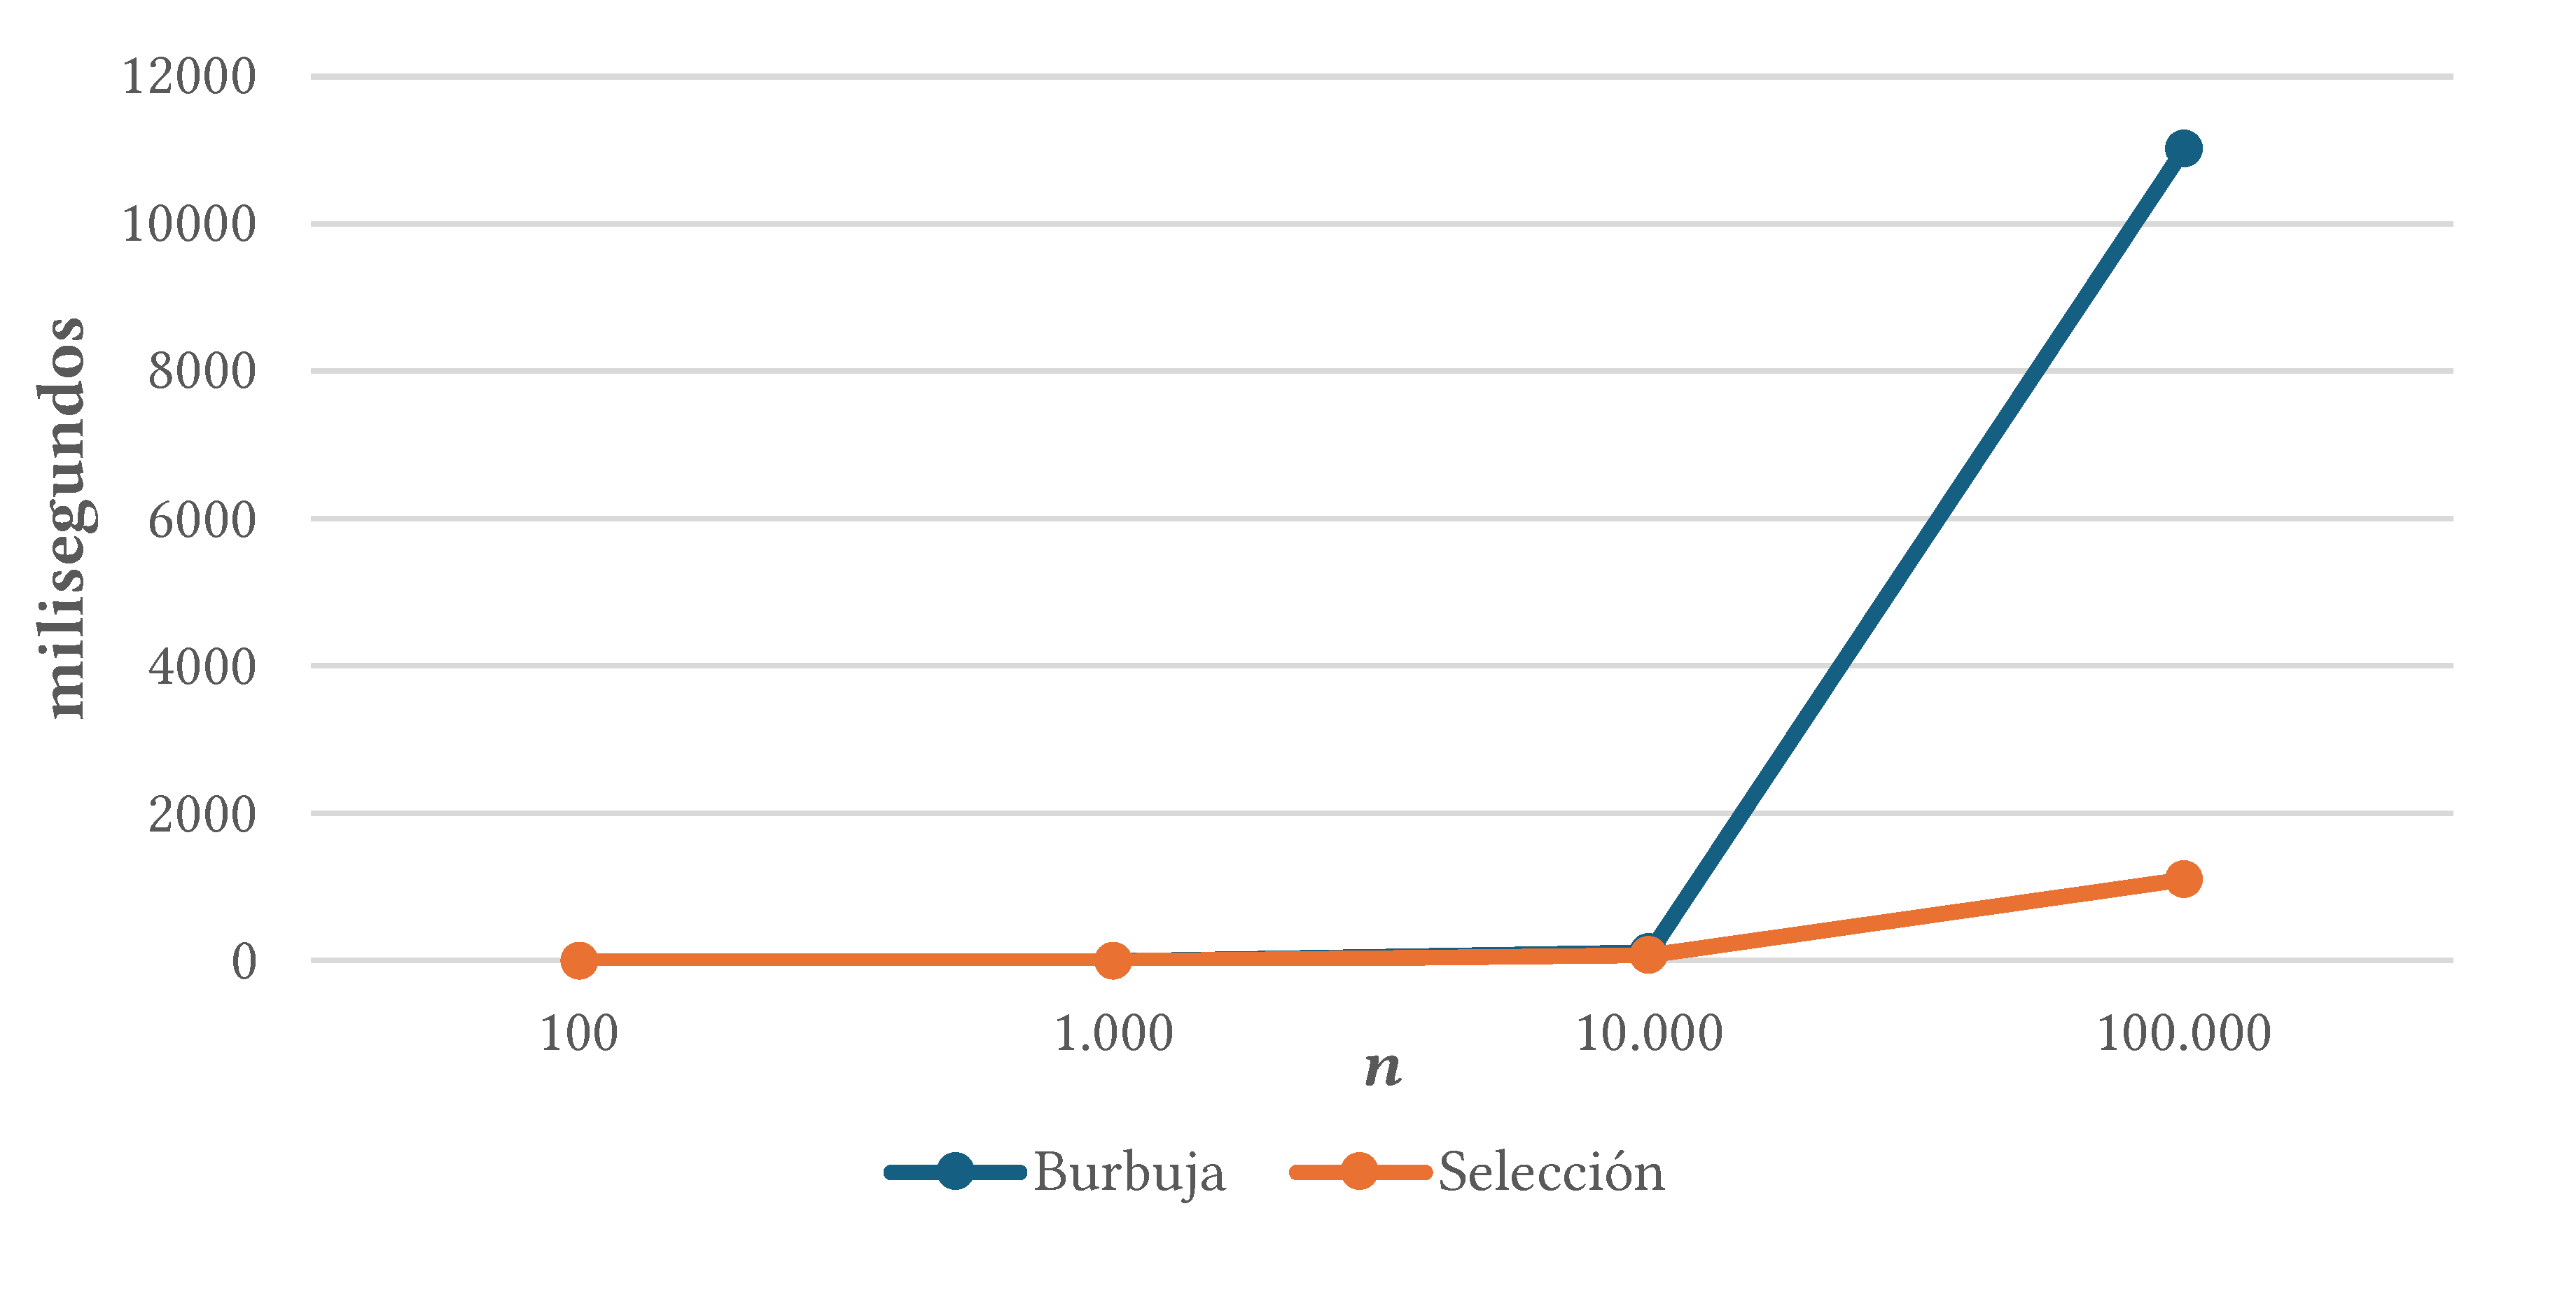
\includegraphics[width=0.78\linewidth]{../resources/practica6/images/tiempos.pdf}
\caption{Comparación de tiempos de ejecución de los algoritmos de burbuja y selección.}\label{fig-p6-tiempos}
\end{figure}

\begin{PracticeWarningBox}{Posible falta de memoria}
Para valores de \(n\) muy grandes, es posible que el programa no tenga suficiente memoria para ejecutar el algoritmo de ordenación de burbuja. Puedes aumentar la memoria asignada a Java desde \texttt{Run > Run Configurations...}, pestaña \texttt{Arguments}, añadiendo \texttt{-Xmx1024m} en \texttt{VM arguments}.
\end{PracticeWarningBox}

\subsection{Medición de tiempo de ejecución}\label{medicion-de-tiempo-de-ejecucion}

Para medir el tiempo de ejecución de cada implementación, utiliza la clase \texttt{System} de Java antes y después de ejecutar el algoritmo:

\PracticeCode{../resources/practica6/snippets/java/timing.java}

\section{Entrega de la solución}\label{entrega-de-la-solucion}

\textbf{Sólo debe realizar la entrega un miembro del grupo.} Sube a Moodle un fichero comprimido \texttt{practica6.zip} que contenga:

\begin{itemize}
\tightlist
\item \texttt{OrdenacionBurbuja.java}: implementación del algoritmo de ordenación de burbuja.
\item \texttt{OrdenacionSeleccion.java}: implementación del algoritmo de ordenación por selección.
\item \texttt{tiempos.xlsx}: archivo de Excel con los tiempos de ejecución medidos para ambos algoritmos y los diferentes tamaños de vector.
\end{itemize}

\end{document}
